\documentclass[english,twoside, openright, hidelinks, 11 pt, class=report,crop=false]{standalone}
\input{../../preamb}



\begin{document}
{\Large Eksamen P1 våren 2025\hfill {\footnotesize Løsning fra \color{blue} \href{https://sindreheggen.wordpress.com/}{OpenMathBooks prosjektet}}}	
\subsection*{Oppgave 1}
$\frac{60}{40}=1,5=150\%$. Sjokoladeplaten er 50\% dyrere på bensinstasjonen enn i butikken.

\subsection*{Oppgave 2}
Den prosentvise fremgangen for henholdsvis Senterpartiet og Arbeiderpartiet er gitt ved brøkene $\frac{5}{20}$ og $\frac{5}{40}$. Da $\frac{5}{20}>\frac{5}{40}$, har Senterpartiet hatt størst fremgang.

\subsection*{Oppgave 3}
Viss $n$ personer skal fordele 100\enh{kr} likt mellom seg, vil prisen $p$ per person være gitt som
\[ p=\frac{100}{n} \] 
Dermed er $p\cdot n=100$, som betyr at $p$ og $n$ er omvendt proporsjonale.
\begin{figure}
	\centering
	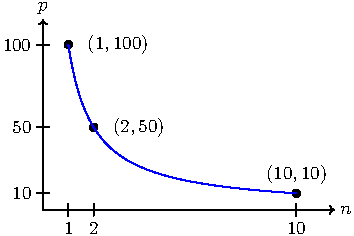
\includegraphics{opg3del1}
\end{figure}
\subsection*{Oppgave 4}
\[ \colb{8}\cdot10^\colb{9}\cdot\colb{1}\cdot10^\colb{0}=8\,000\,000\,000 \]
\[ \colb{4}\cdot10^\colb{3}\cdot\colb{2}\cdot10^\colb{6}=8\,000\,000\,000 \]

\subsection*{Oppgave 5}
Det blir 5\,307\,000\,000\,000 blodceller til sammen.

\subsection*{Oppgave 6}
\abc{
\item I figur 5 får vi 6 kvadrat på skrå, 5 kvadrat loddrett og 25 kvadrat i rutenettet. Altså vil det være 36 kvadrat i figur 5.
\item Skrå kvadrat: $n+1$ \\
Loddrette kvadrat: $n$ \\
Kvadrat i rutenett: $n^2$
\[ \text{Kvadrat i figur $n$}=n+1+n+n^2=n^2+2n+1=(n+1)^2 \]
}

\subsection*{Oppgave 7}
Programmet forteller at Lars årlig vil sette inn 24\,000\enh{kr} på sparekontoen sin. Verdien til \texttt{vekstfaktor} forteller at den årlige sparerenten er 5,8\%. \os

Verdiene som blir printet forteller antall år med sparing, og hvor mye penger det er på konto for hvert år.

\subsection*{Oppgave 8}
\abc{
\item Vi har at
\[ a=\frac{270-90}{20-5}=\frac{180}{15}=12 \]
\textbf{Alternativ 1 for å finne $\bm b$}\\
Av punktet $(5, 90)$ har vi at
\begin{align*}
	12\cdot5+b&=90 \\
	b &= 90-60\\
	b&=30
\end{align*}
\textbf{Alternativ 2 for å finne $\bm b$}\\
Da $G(0)=b$, har vi at
\begin{align*}
	\frac{90-b}{5-0}&=12 \\
	90-b &= 60 \\
	b&=30
\end{align*}
\textbf{Alternativ 3 for å finne $\bm b$}\\
Vi starter i punktet $(5, 90)$, og går 12 ned for hver gang vi går 1 til venstre på grafen. Når $x=0$, er $y=b=30$ \vsk

Altså er 
\[ g(x)=12x+30 \]
\item Det er rimelig å anta at godteriet har en fast hektopris, og at bøtta har en fast pris. Da koster godteriet 12\enh{kr/hg} og bøtta koster 30\enh{kr}.
\item 
\[ G(8)=12\cdot8+30=96+30=126 \]
En bøtte med 8\enh{hg} godteri koster 126\enh{kr}. 
}
\newpage
\subsection*{Oppgave 1}
\abc{
\item Skriver inn punktene i et regneark i GeoGebra, lager en liste av punktene, og bruker kommandoen \texttt{RegEksp}. Får da samme $K$ som i oppgaveteksten.
\item 1,2 er vekstfaktoren til $K$. For hver måned som går, øker $K$ med 20\%.
\item Bruker kommandoen \texttt{Linje}, og får en linje med stigningstall $70,2$. Dette betyr at den gjennomsnittlige økningen av antall smittede mellom $x=4$ og $x=21$ er lik $70,2$.
\item Mai i 2025 tilsvarer $x=29$. Bruker kommandoen \texttt{K(29)}, og får at det da (avrundet) vil være $5336$ tilfeller.
\begin{figure}
	
\includegraphics[scale=0.22]{opg1}
\end{figure}
}
\subsection*{Oppgave 2}
\abc{
\item $\frac{3\,300\,000}{40\,000}=82,5$. Hver deltaker har i gjennomsnitt gått 82,5\enh{km}.
\item $\frac{3\,300\,000}{83}\approx39\,759$. Der har regnet at det er ca 39\,759\enh{km} rundt jorda.
}
\newpage
\subsection*{Oppgave 3}
Vi lar $x$ være antall aviser solgt. Da viser $f$ Tilbud 1 og $g$ viser Tilbud 2. Bruker kommandoen \texttt{Skjæring} for å finne at $f$ får høyere verdi enn $g$ fra og med 21 solgte aviser.\os
Hvis Elise tror hun vil greie å selge 21 eller flere aviser bør hun altså velge Tilbud 1. Hvis ikke bør hun velge Tilbud 2.
\begin{figure}
	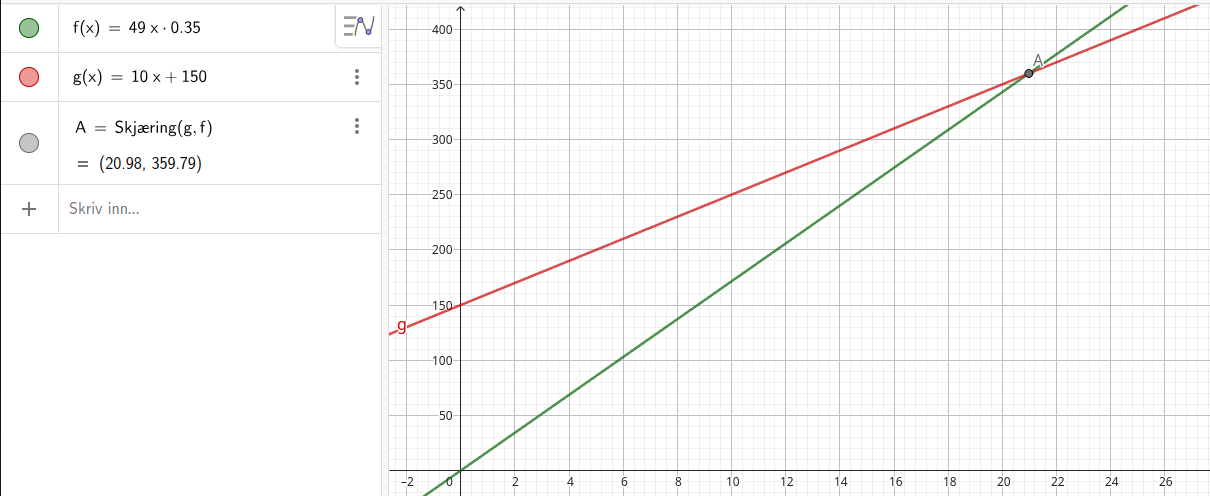
\includegraphics[scale=0.3]{opg3}
\end{figure}
\subsection*{Oppgave 4}
Hvis vi setter original pris på fire aviser lik $x$, må vi ha at
\begin{align}
	x\cdot0,51&=99 \\
	x&=\frac{99}{0,51} \\
	&\approx 194
\end{align}
$\frac{194}{4}=48,5$. En avis koster altså 48,5\enh{kr}.
\subsection*{Oppgave 5}
\textbf{Furu 28x145}\\
$145\enh{mm}=0,145\enh{m}$. Ved å kjøpe 1\enh{m} får vi en overflate lik 0,145$\enh{m}^2$. $\frac{67,9}{0,145}\approx468$. Prisen per kvadratmeter er ca. 468\enh{kr}.\vsk

\textbf{Furu 28x095}\\
$\frac{49,9}{0,095}\approx525$. Prisen per kvadratmeter er ca. 525\enh{kr}.

\newpage
\subsection*{Oppgave 6}
\abc{
\item Vi får formelen 
\[ h=\frac{V}{\pi r^2}=\frac{450}{\pi r^2} \]
\begin{figure}
	\centering
	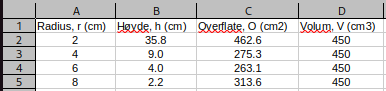
\includegraphics[scale=0.5]{opg6a} \\
	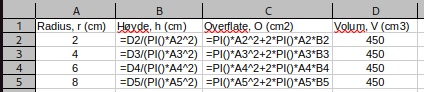
\includegraphics[scale=0.5]{opg6aa}
\end{figure}
\item Av uttrykket vi fant i oppgave a) og uttrykket for $O$ har vi at
\[ O(r)=\pi r^2 + 2\pi r \frac{450}{\pi r^2}=\pi r^2+\frac{900}{r} \]
Grafen til $O$ er vist i GeoGebra (se figur under).
\item Av grafen ser vi at bunnpunktet ligger mellom $r=0$ og $r=10$. Bruker kommandoen \texttt{Ekstremalpunkt}, og finner at $O$ er minst når $r=5,23$ (cm). Da er $O\approx258$ ($\text{cm}^3$).
}
\begin{figure}
	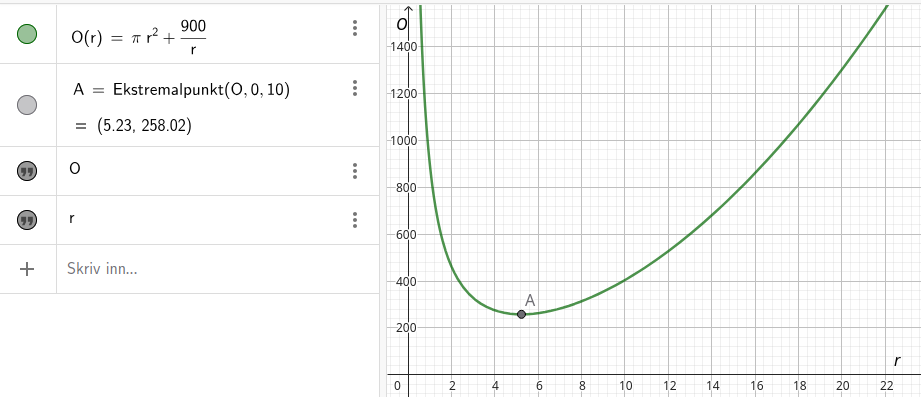
\includegraphics[scale=0.4]{opg6bc}
\end{figure}
\newpage
\subsection*{Oppgave 7}
Ut ifra antakelsene gitt i tabellen under, vil en hjemmelaget baguett koste ca 30 kr (D8). Det betyr at Sofie sparer 35\enh{kr} per dag. Det er minst $5\cdot4=20$ skoledager i løpet av en måned, altså kan Sofie spare $(35\cdot20)\enh{kr}=700\enh{kr}$ i måneden.
\begin{figure}
	\centering
	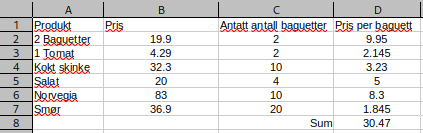
\includegraphics[scale=0.5]{opg7a}
	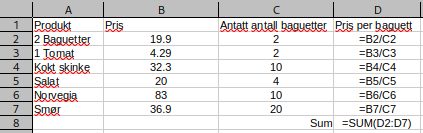
\includegraphics[scale=0.5]{opg7b}
\end{figure}
\end{document}